\begin{figure}[htbp]
\centering



\tikzset{every picture/.style={line width=0.75pt}} %set default line width to 0.75pt        

\begin{tikzpicture}[x=0.75pt,y=0.75pt,yscale=-1,xscale=1]
%uncomment if require: \path (0,787.8333282470703); %set diagram left start at 0, and has height of 787.8333282470703

%Straight Lines [id:da8347099233381158] 
\draw [line width=2.25]    (470,484.83) -- (581,484.83) ;


%Rounded Rect [id:dp009535500915653694] 
\draw  [fill={rgb, 255:red, 203; green, 239; blue, 229 }  ,fill opacity=1 ] (10,419.38) .. controls (10,392.6) and (31.71,370.9) .. (58.49,370.9) -- (459.51,370.9) .. controls (486.29,370.9) and (508,392.6) .. (508,419.38) -- (508,564.85) .. controls (508,591.62) and (486.29,613.33) .. (459.51,613.33) -- (58.49,613.33) .. controls (31.71,613.33) and (10,591.62) .. (10,564.85) -- cycle ;
%Shape: Polygon Curved [id:ds3945329006458995] 
\draw  [color={rgb, 255:red, 242; green, 175; blue, 175 }  ,draw opacity=1 ][line width=3]  (118,440.33) .. controls (127,360.33) and (496,391.33) .. (488,413.33) .. controls (480,435.33) and (515,589.33) .. (438,578.33) .. controls (361,567.33) and (410,518.33) .. (390,488.33) .. controls (370,458.33) and (109,520.33) .. (118,440.33) -- cycle ;
%Rounded Rect [id:dp3266494529696595] 
\draw  [fill={rgb, 255:red, 242; green, 175; blue, 175 }  ,fill opacity=1 ] (247,203.23) .. controls (247,192.98) and (255.31,184.67) .. (265.57,184.67) -- (486.43,184.67) .. controls (496.69,184.67) and (505,192.98) .. (505,203.23) -- (505,258.93) .. controls (505,269.19) and (496.69,277.5) .. (486.43,277.5) -- (265.57,277.5) .. controls (255.31,277.5) and (247,269.19) .. (247,258.93) -- cycle ;

%Straight Lines [id:da5480959124322587] 
\draw [line width=1.5]  [dash pattern={on 1.69pt off 2.76pt}]  (277,233.33) -- (470,232.33) ;


%Image [id:dp7552041287953648] 
\draw (365,243.5) node  {
\includegraphics[width=52.5pt,height=52.5pt]{figures/router-29825_1280.pdf}};
%Image [id:dp9413637243735231] 
\draw (459,243.5) node  {
\includegraphics[width=52.5pt,height=52.5pt]{figures/router-29825_1280.pdf}};
%Image [id:dp785651084861142] 
\draw (281,243.5) node  {
\includegraphics[width=52.5pt,height=52.5pt]{figures/router-29825_1280.pdf}};
%Rounded Rect [id:dp3607470454038808] 
\draw  [fill={rgb, 255:red, 255; green, 248; blue, 177 }  ,fill opacity=1 ] (6,116.8) .. controls (6,95.37) and (23.37,78) .. (44.8,78) -- (176.2,78) .. controls (197.63,78) and (215,95.37) .. (215,116.8) -- (215,233.2) .. controls (215,254.63) and (197.63,272) .. (176.2,272) -- (44.8,272) .. controls (23.37,272) and (6,254.63) .. (6,233.2) -- cycle ;

%Straight Lines [id:da6281461745789373] 
\draw [line width=1.5]  [dash pattern={on 1.69pt off 2.76pt}]  (45,130.33) -- (120,230.33) ;


%Straight Lines [id:da1553743343202807] 
\draw [line width=1.5]  [dash pattern={on 1.69pt off 2.76pt}]  (45,130.33) -- (181,131.33) ;


%Straight Lines [id:da7040489254906964] 
\draw [line width=1.5]  [dash pattern={on 1.69pt off 2.76pt}]  (119,229.33) -- (180,130.33) ;


%Image [id:dp41322551228030835] 
\draw (42.5,145) node  {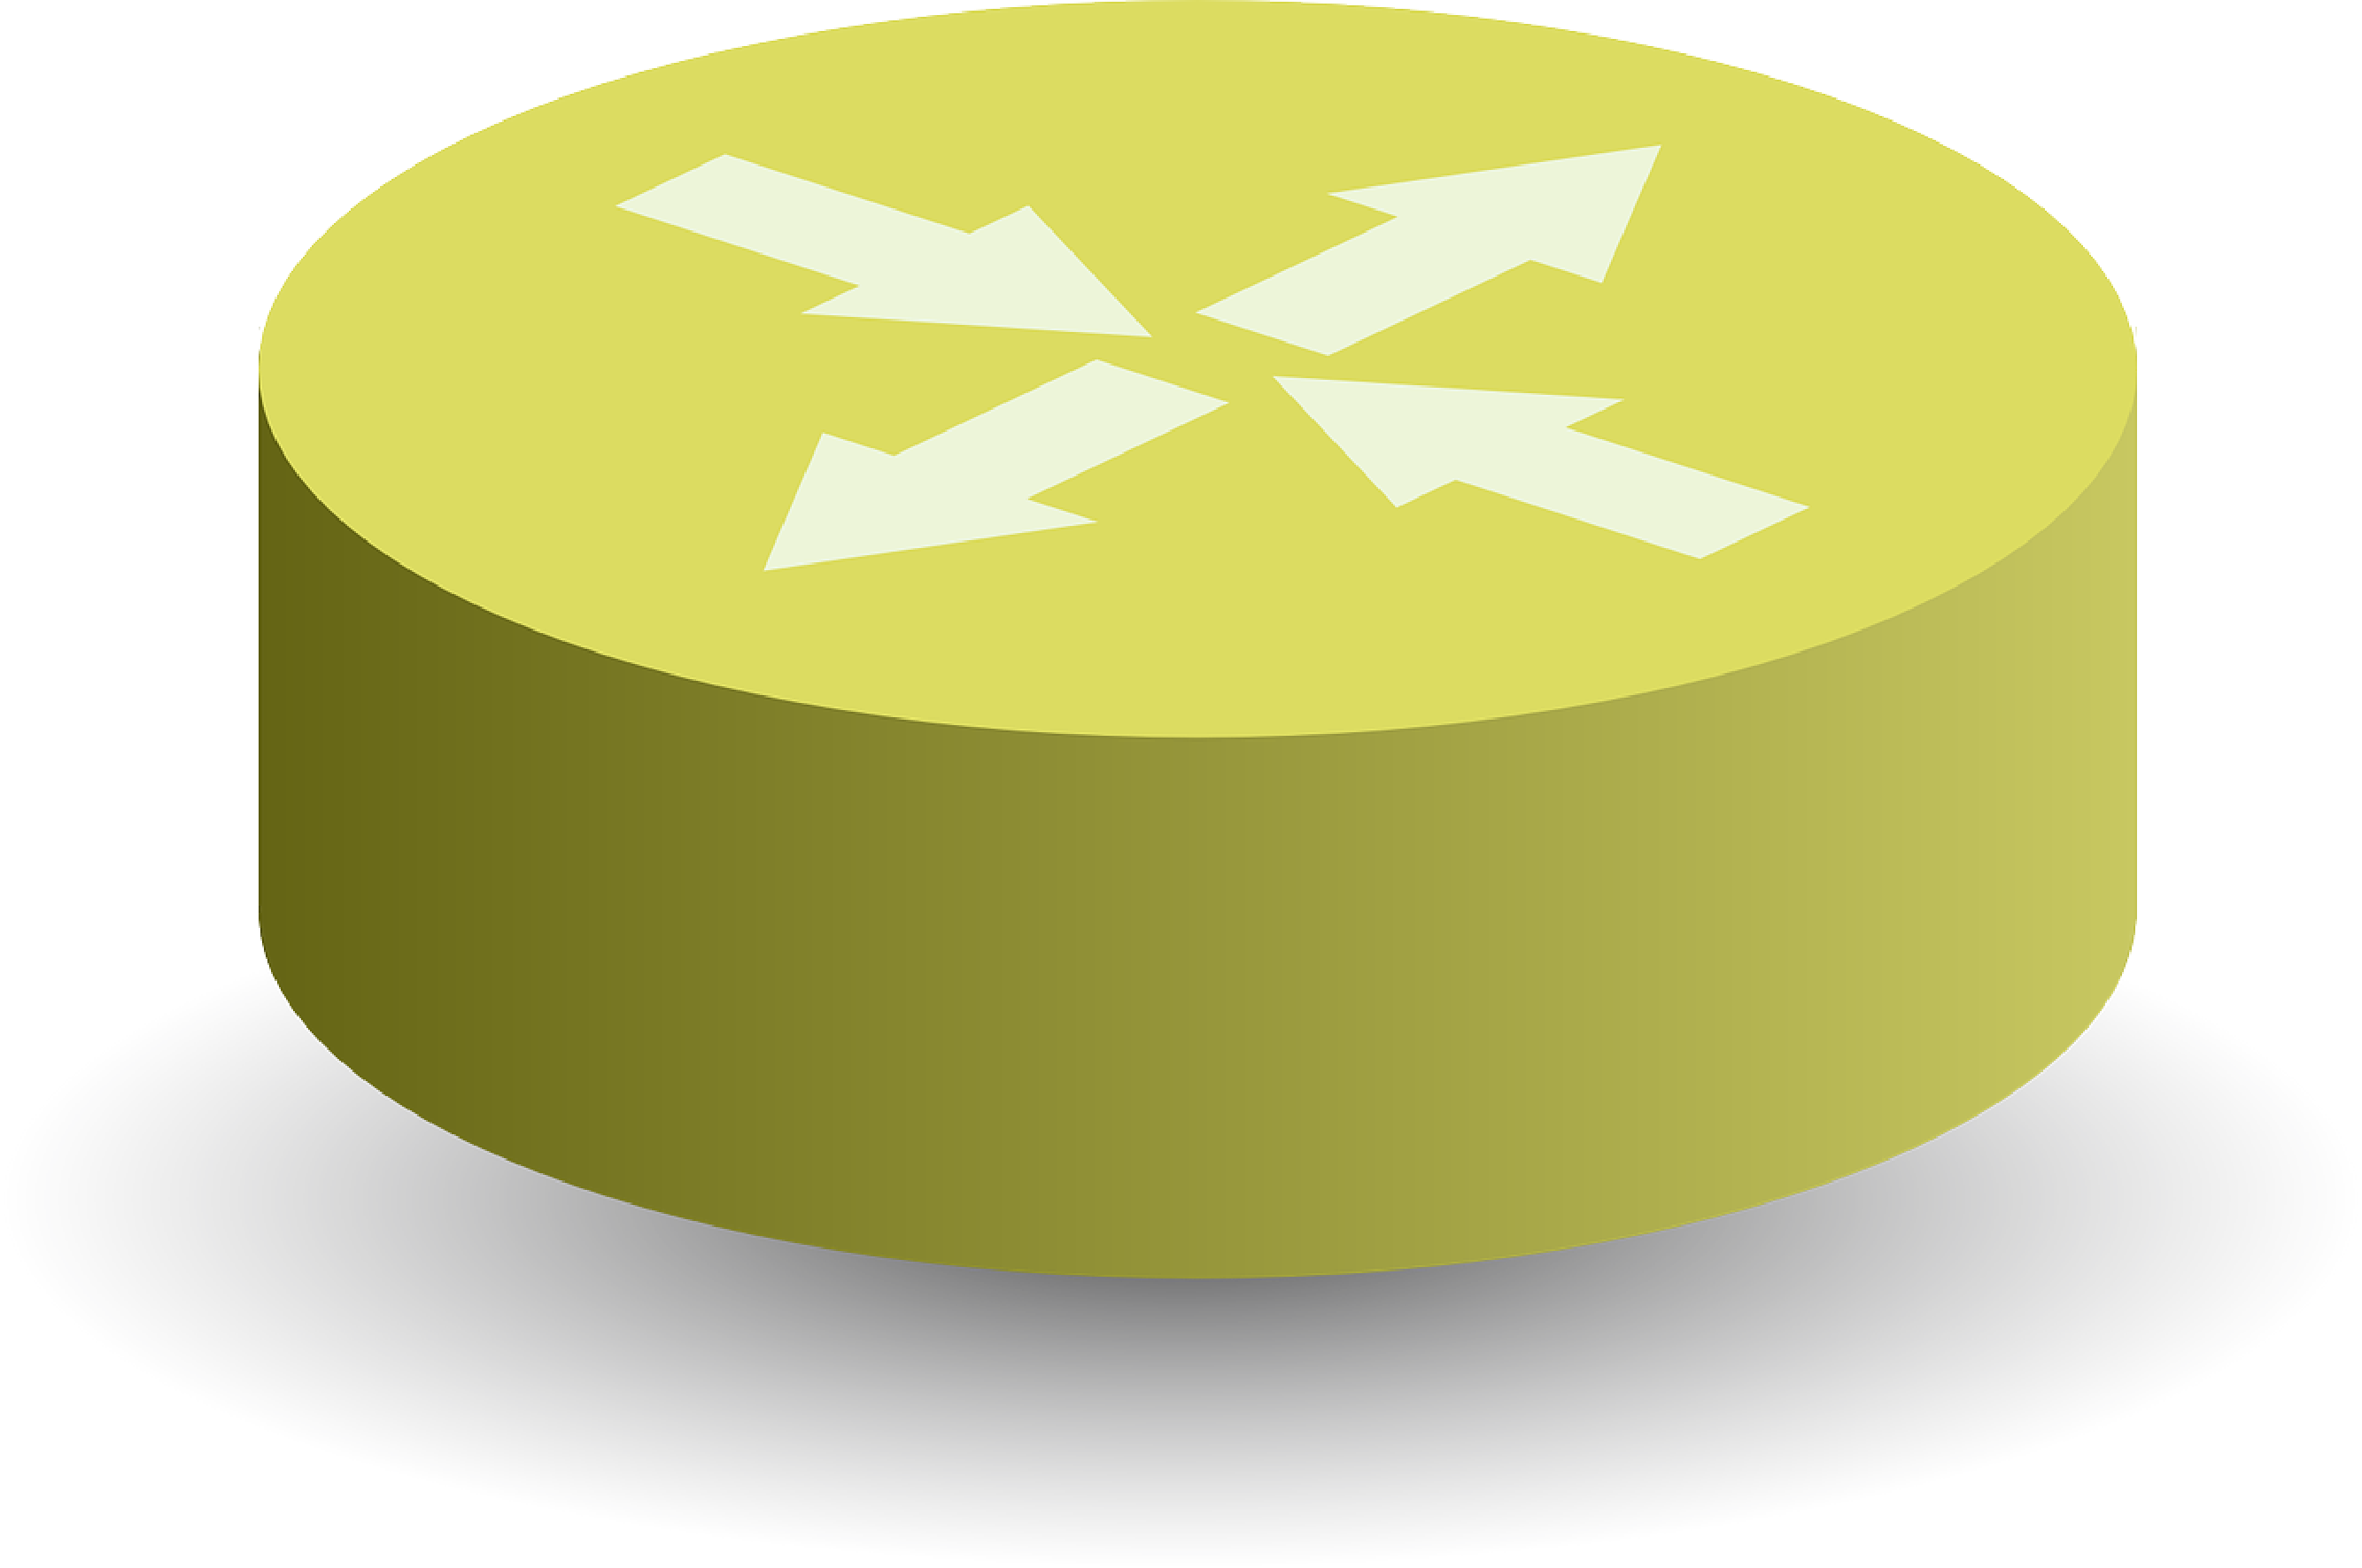
\includegraphics[width=52.5pt,height=52.5pt]{figures/router-158644_1280.pdf}};
%Image [id:dp16387001457338324] 
\draw (177.5,145) node  {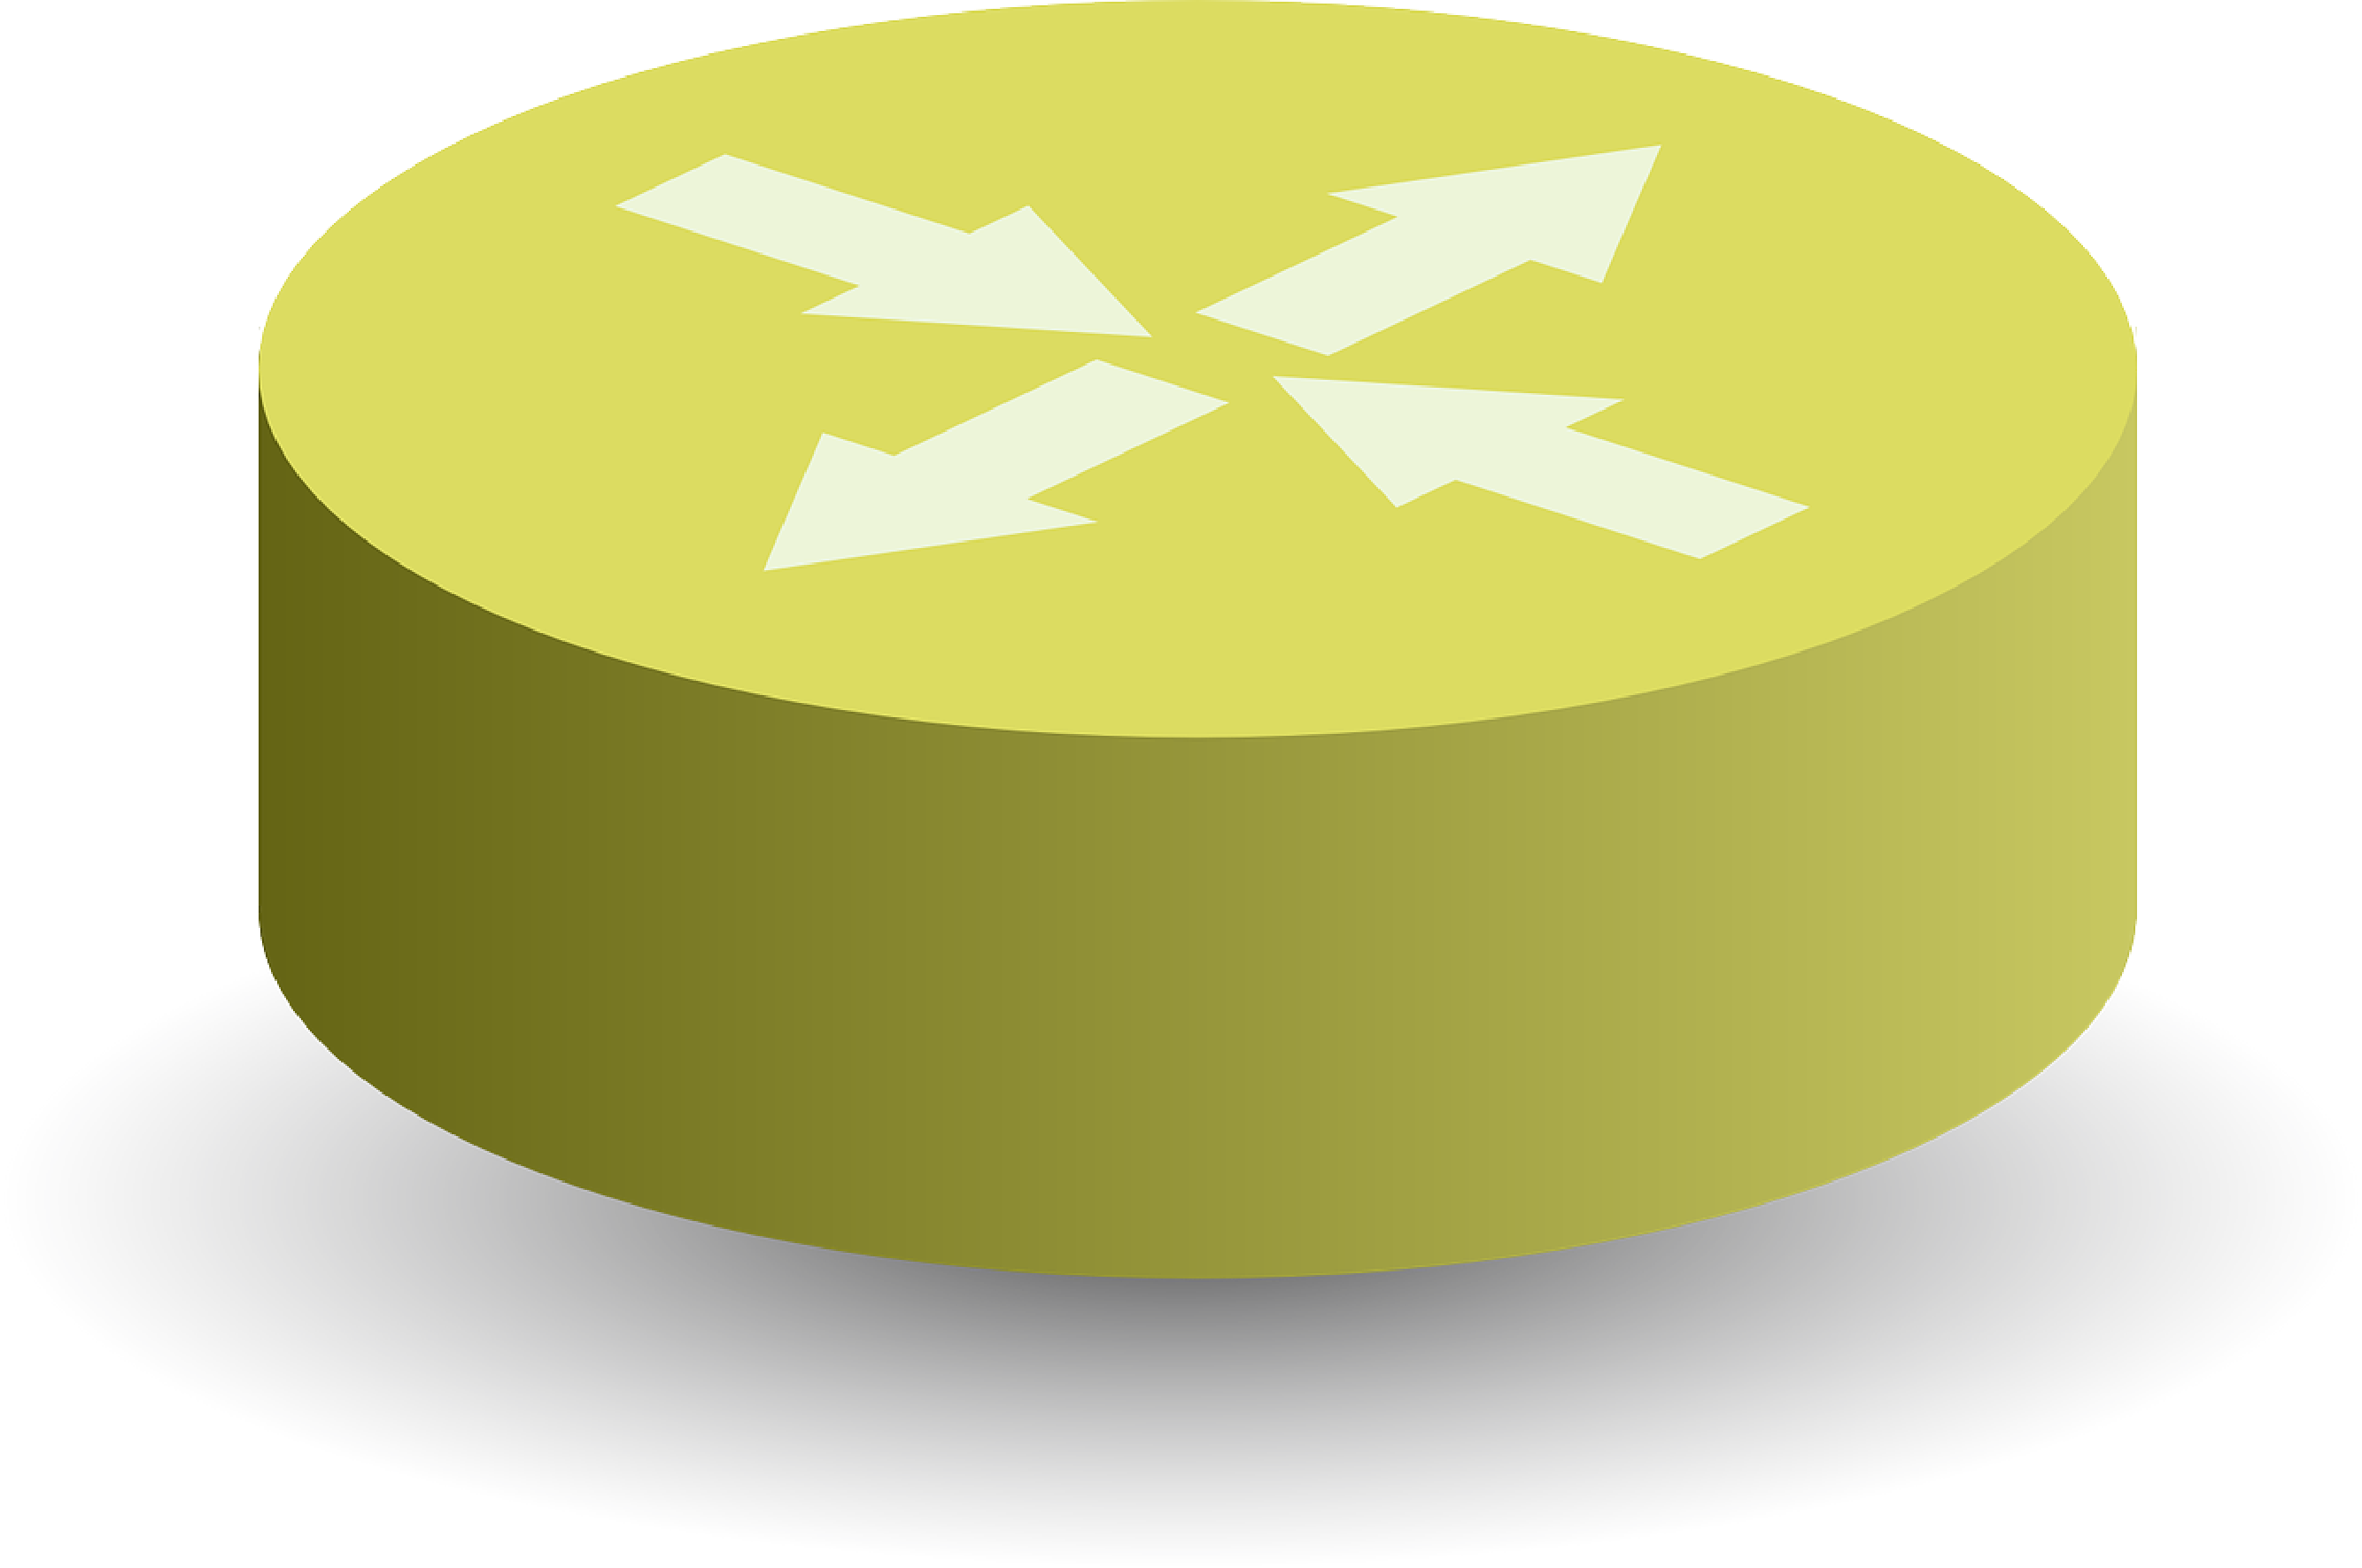
\includegraphics[width=52.5pt,height=52.5pt]{figures/router-158644_1280.pdf}};
%Image [id:dp1012276528015783] 
\draw (111.5,236.5) node  {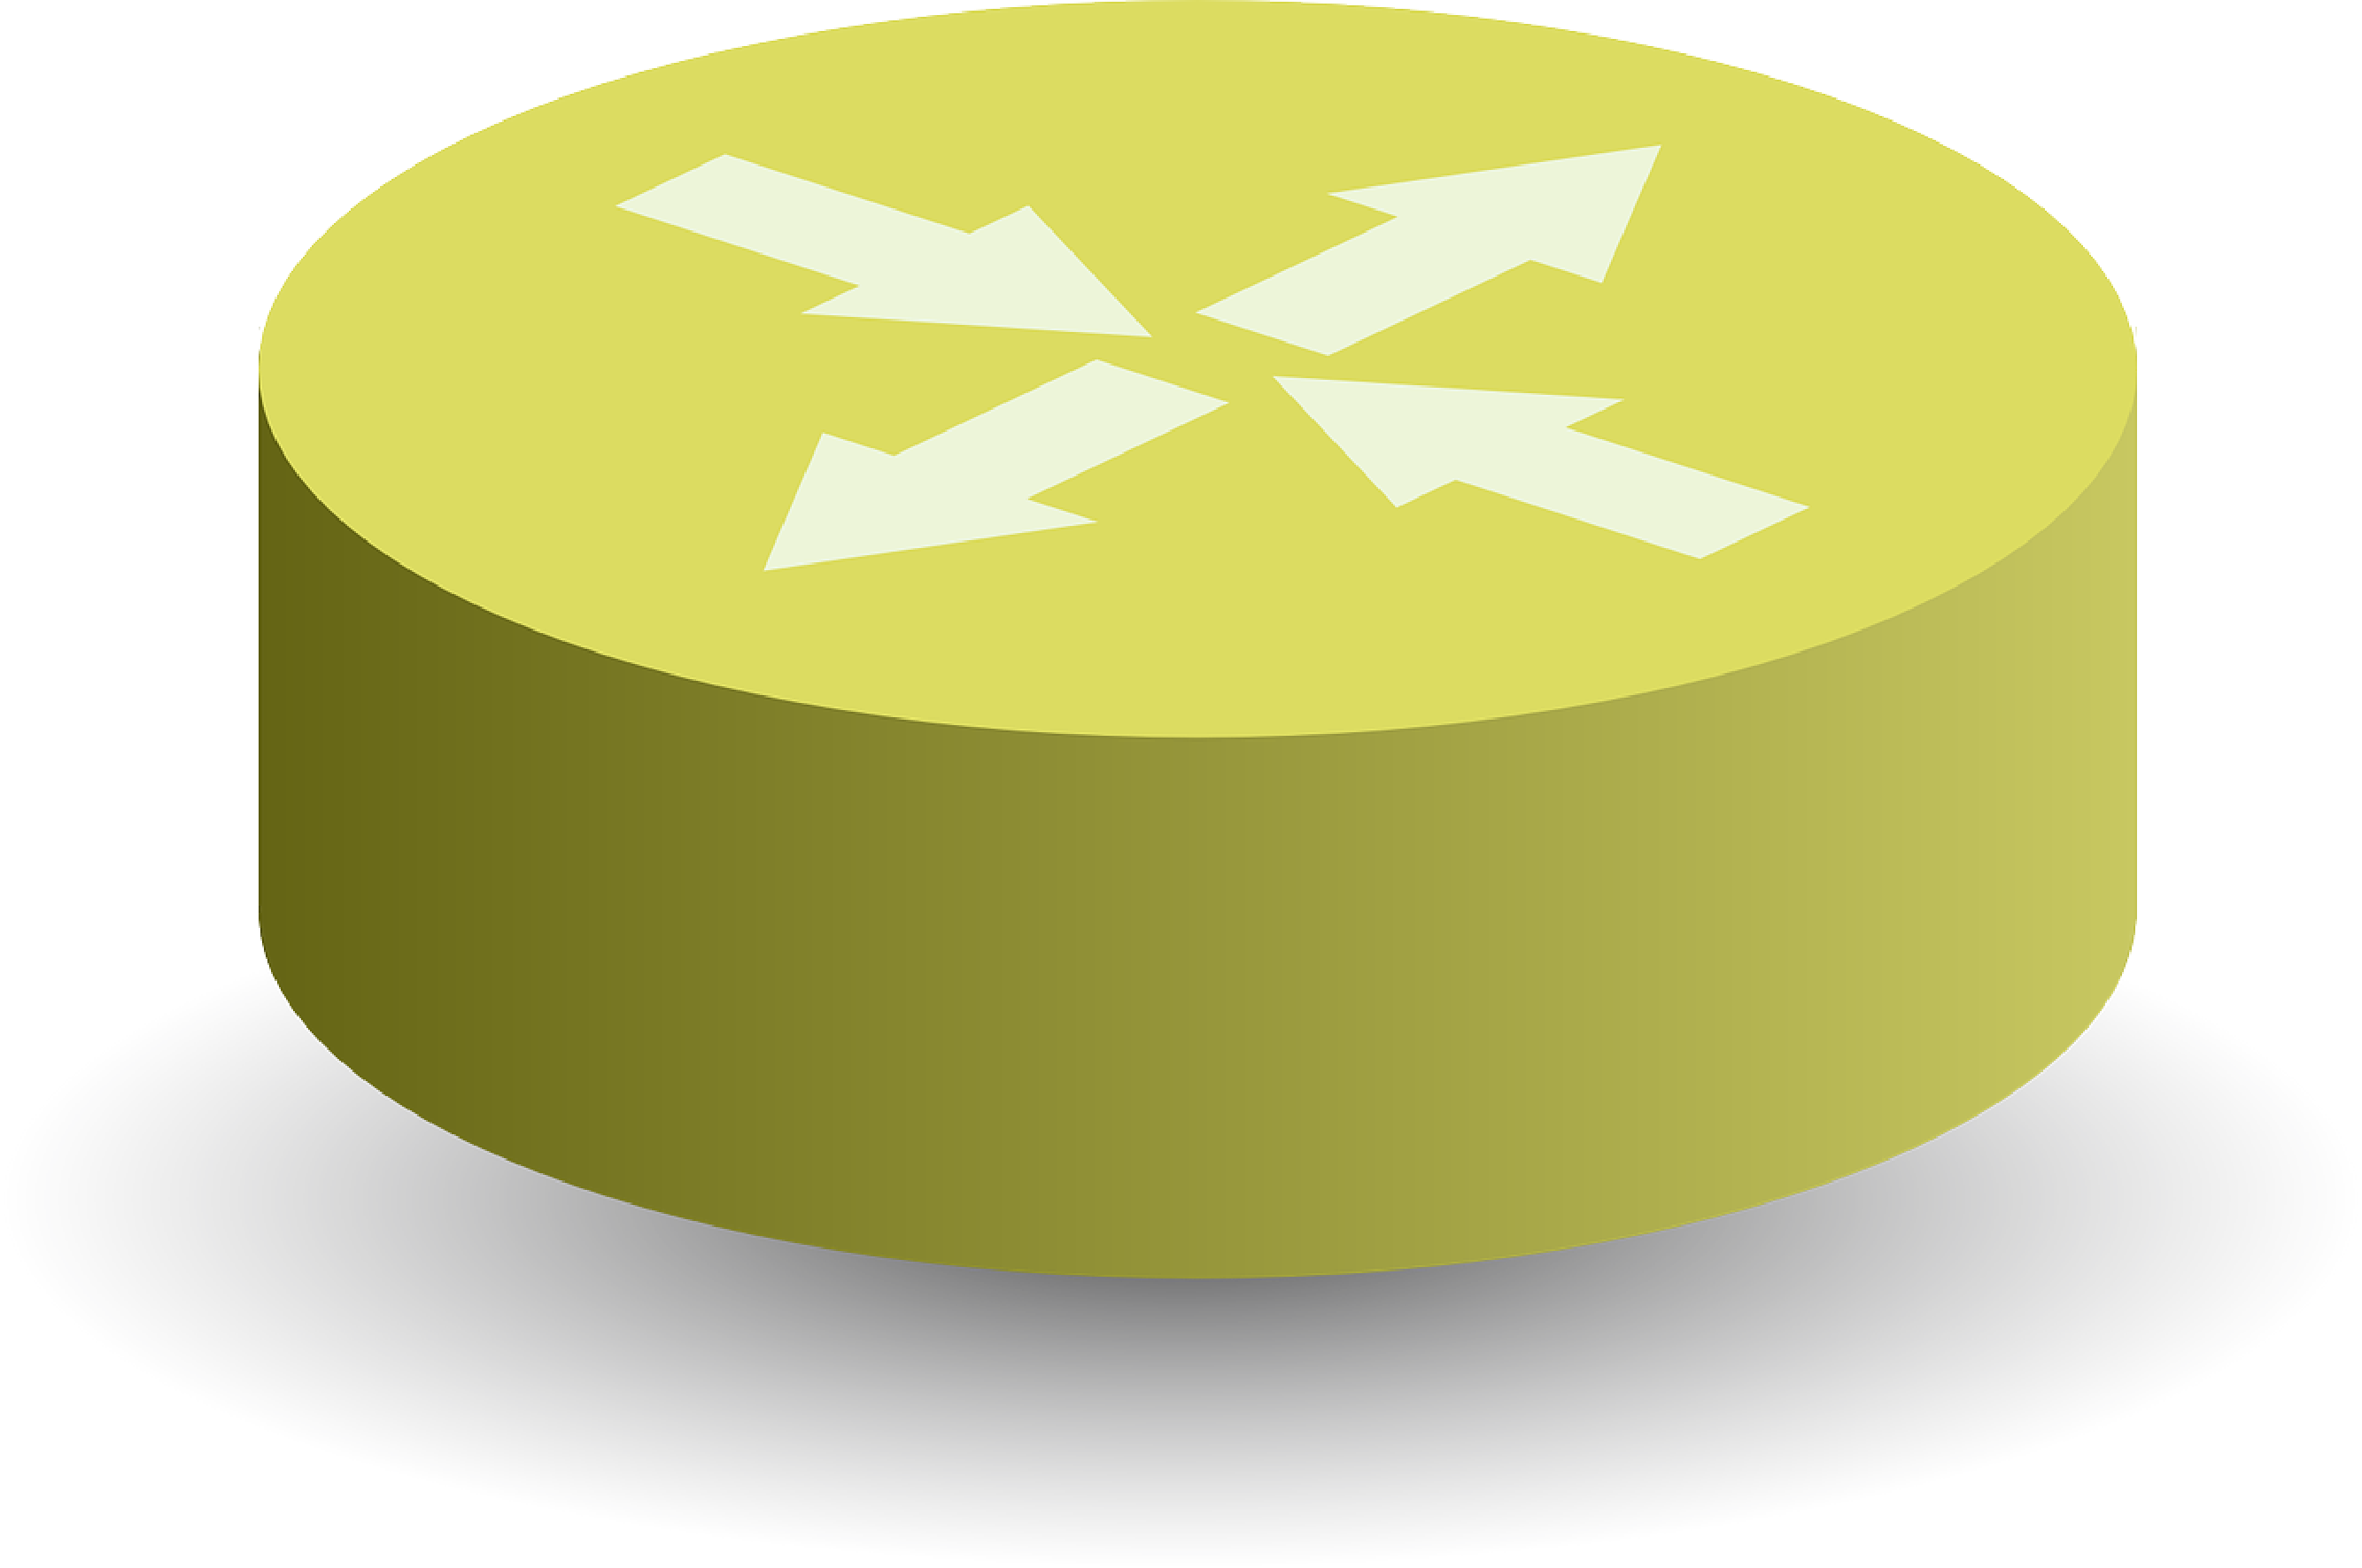
\includegraphics[width=52.5pt,height=52.5pt]{figures/router-158644_1280.pdf}};
%Straight Lines [id:da10827340921387374] 
\draw    (67,469.33) -- (180,428.33) ;


%Straight Lines [id:da02465044628511004] 
\draw    (67,469.33) -- (182,526.33) ;


%Straight Lines [id:da7232328020483667] 
\draw    (179,526.33) -- (177,428.33) ;


%Straight Lines [id:da6335138571596731] 
\draw    (440,530.33) -- (438,432.33) ;


%Straight Lines [id:da5081473547182844] 
\draw    (186,435.33) -- (462,436.33) ;


%Straight Lines [id:da5273919871085183] 
\draw    (185,530.33) -- (461,531.33) ;


%Image [id:dp10904051335047615] 
\draw (68,484.5) node  {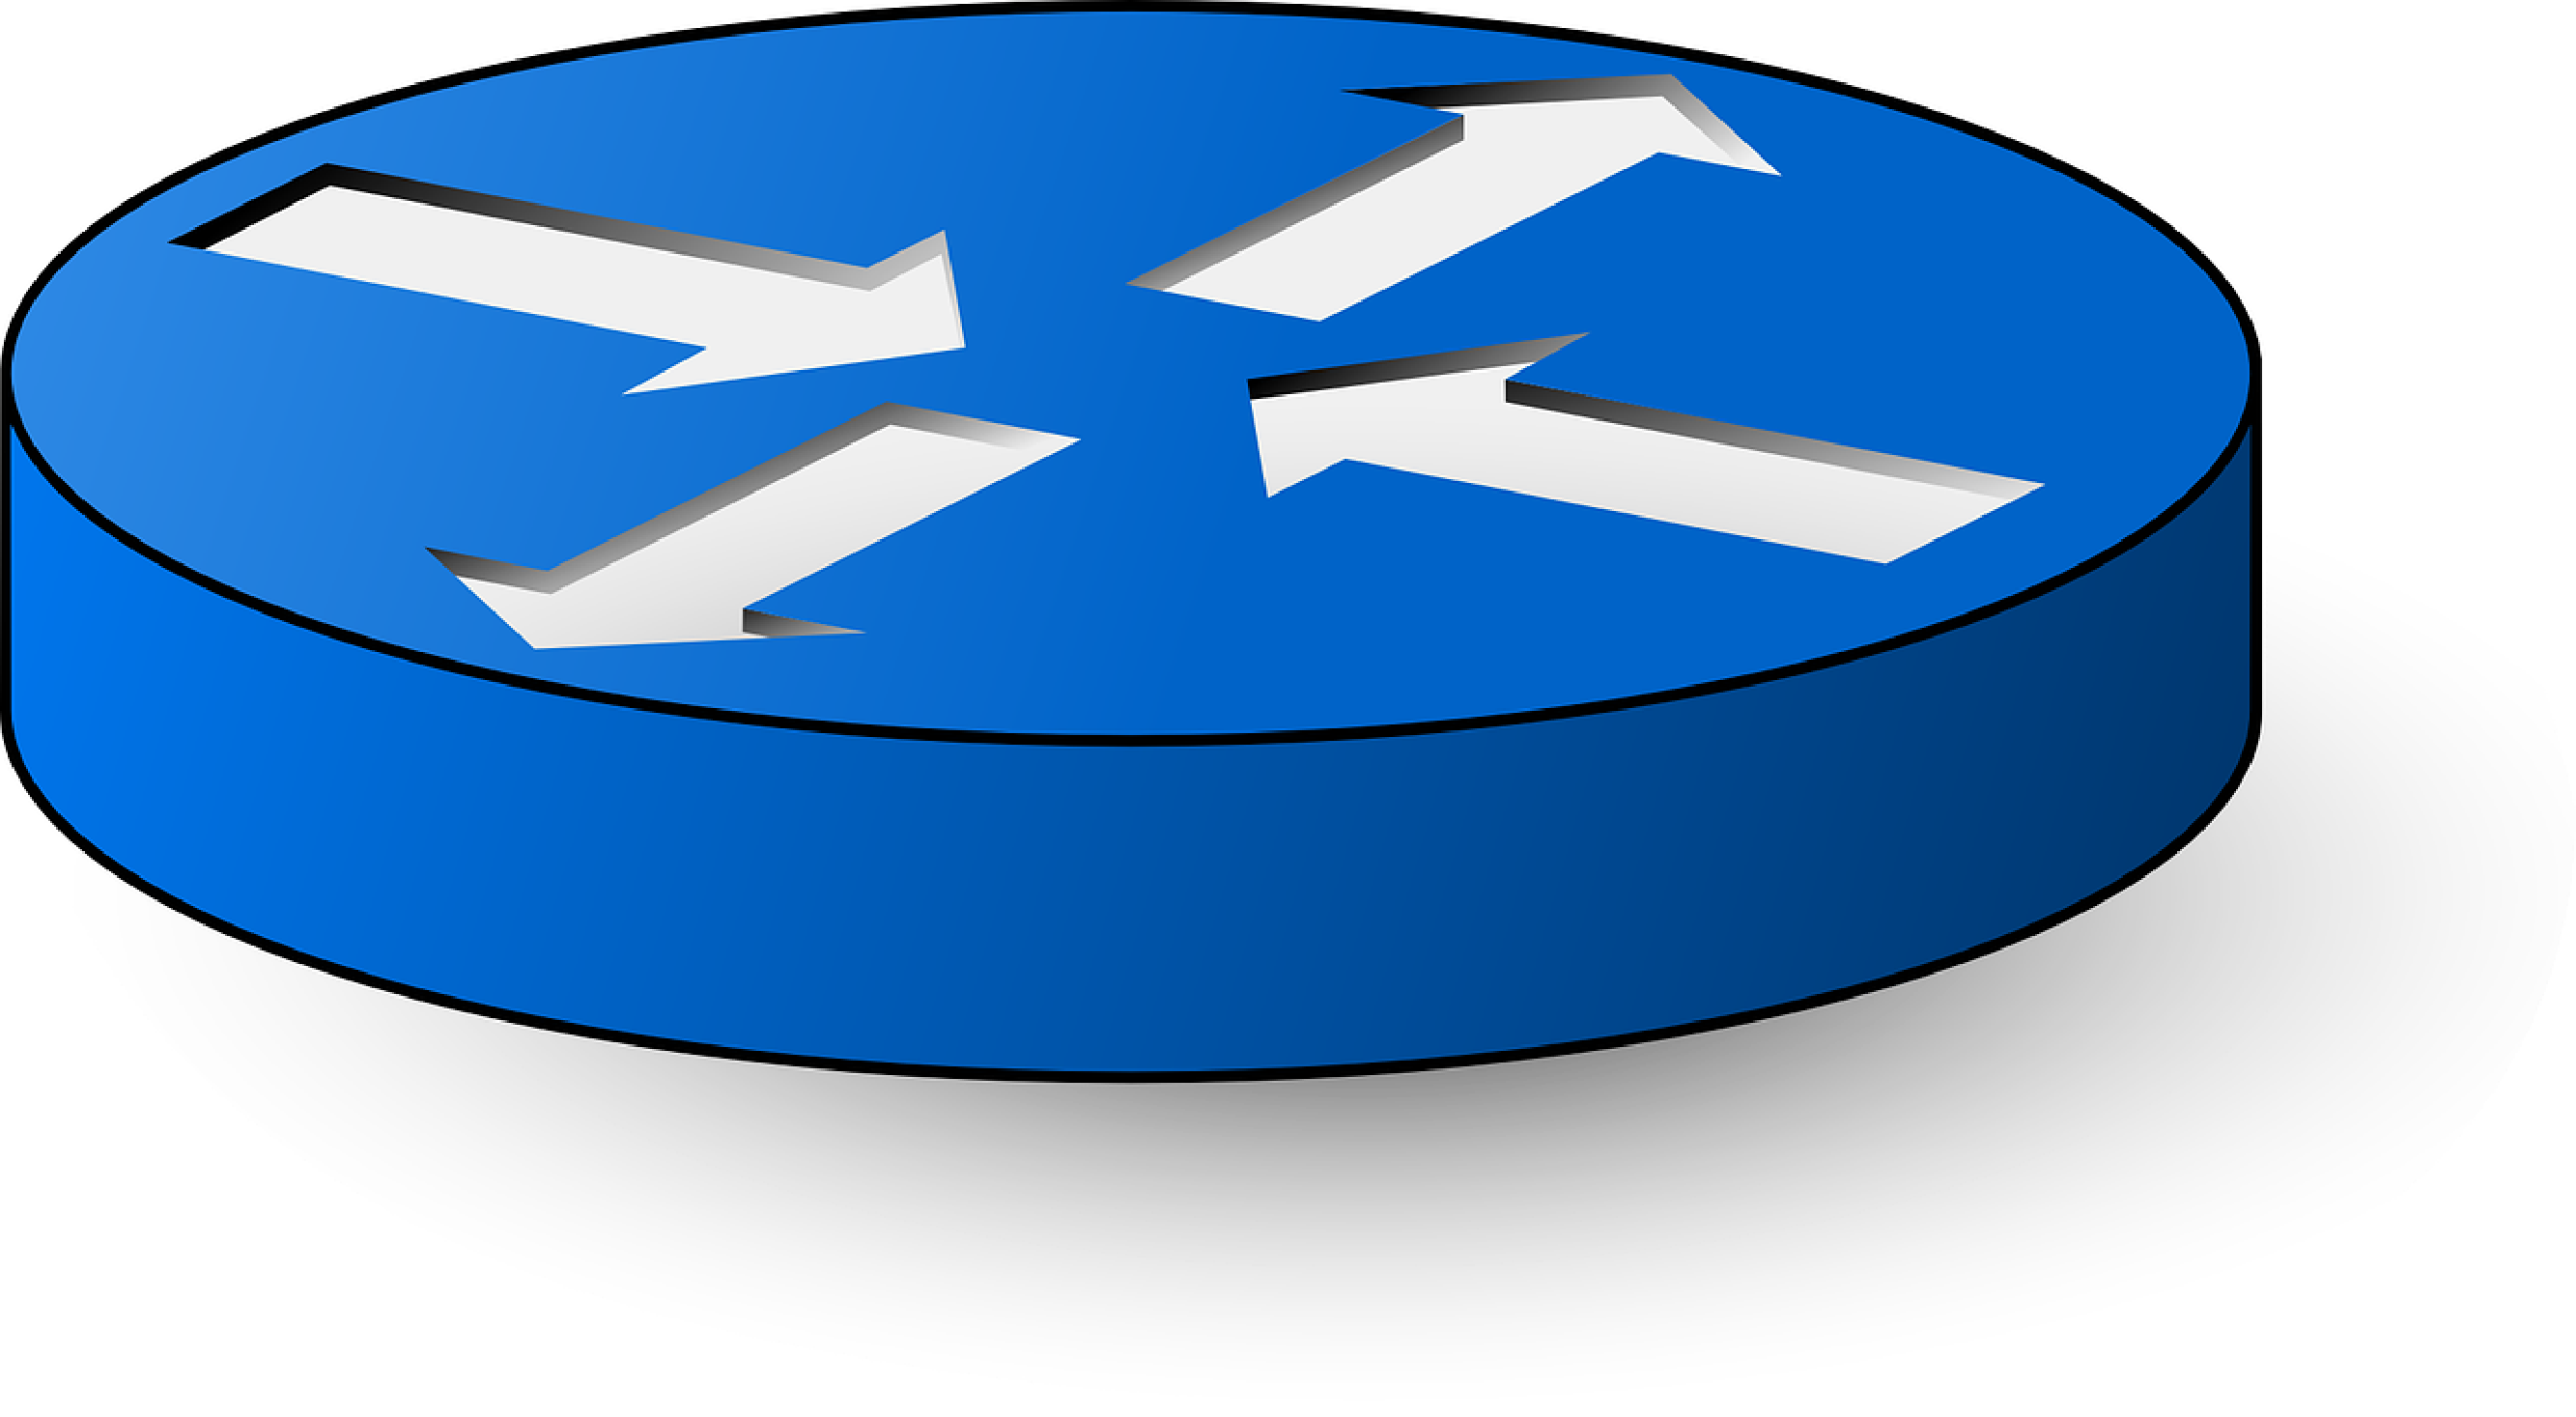
\includegraphics[width=52.5pt,height=52.5pt]{figures/router-30140_1280.pdf}};
%Image [id:dp7146163070755307] 
\draw (185,444.5) node  {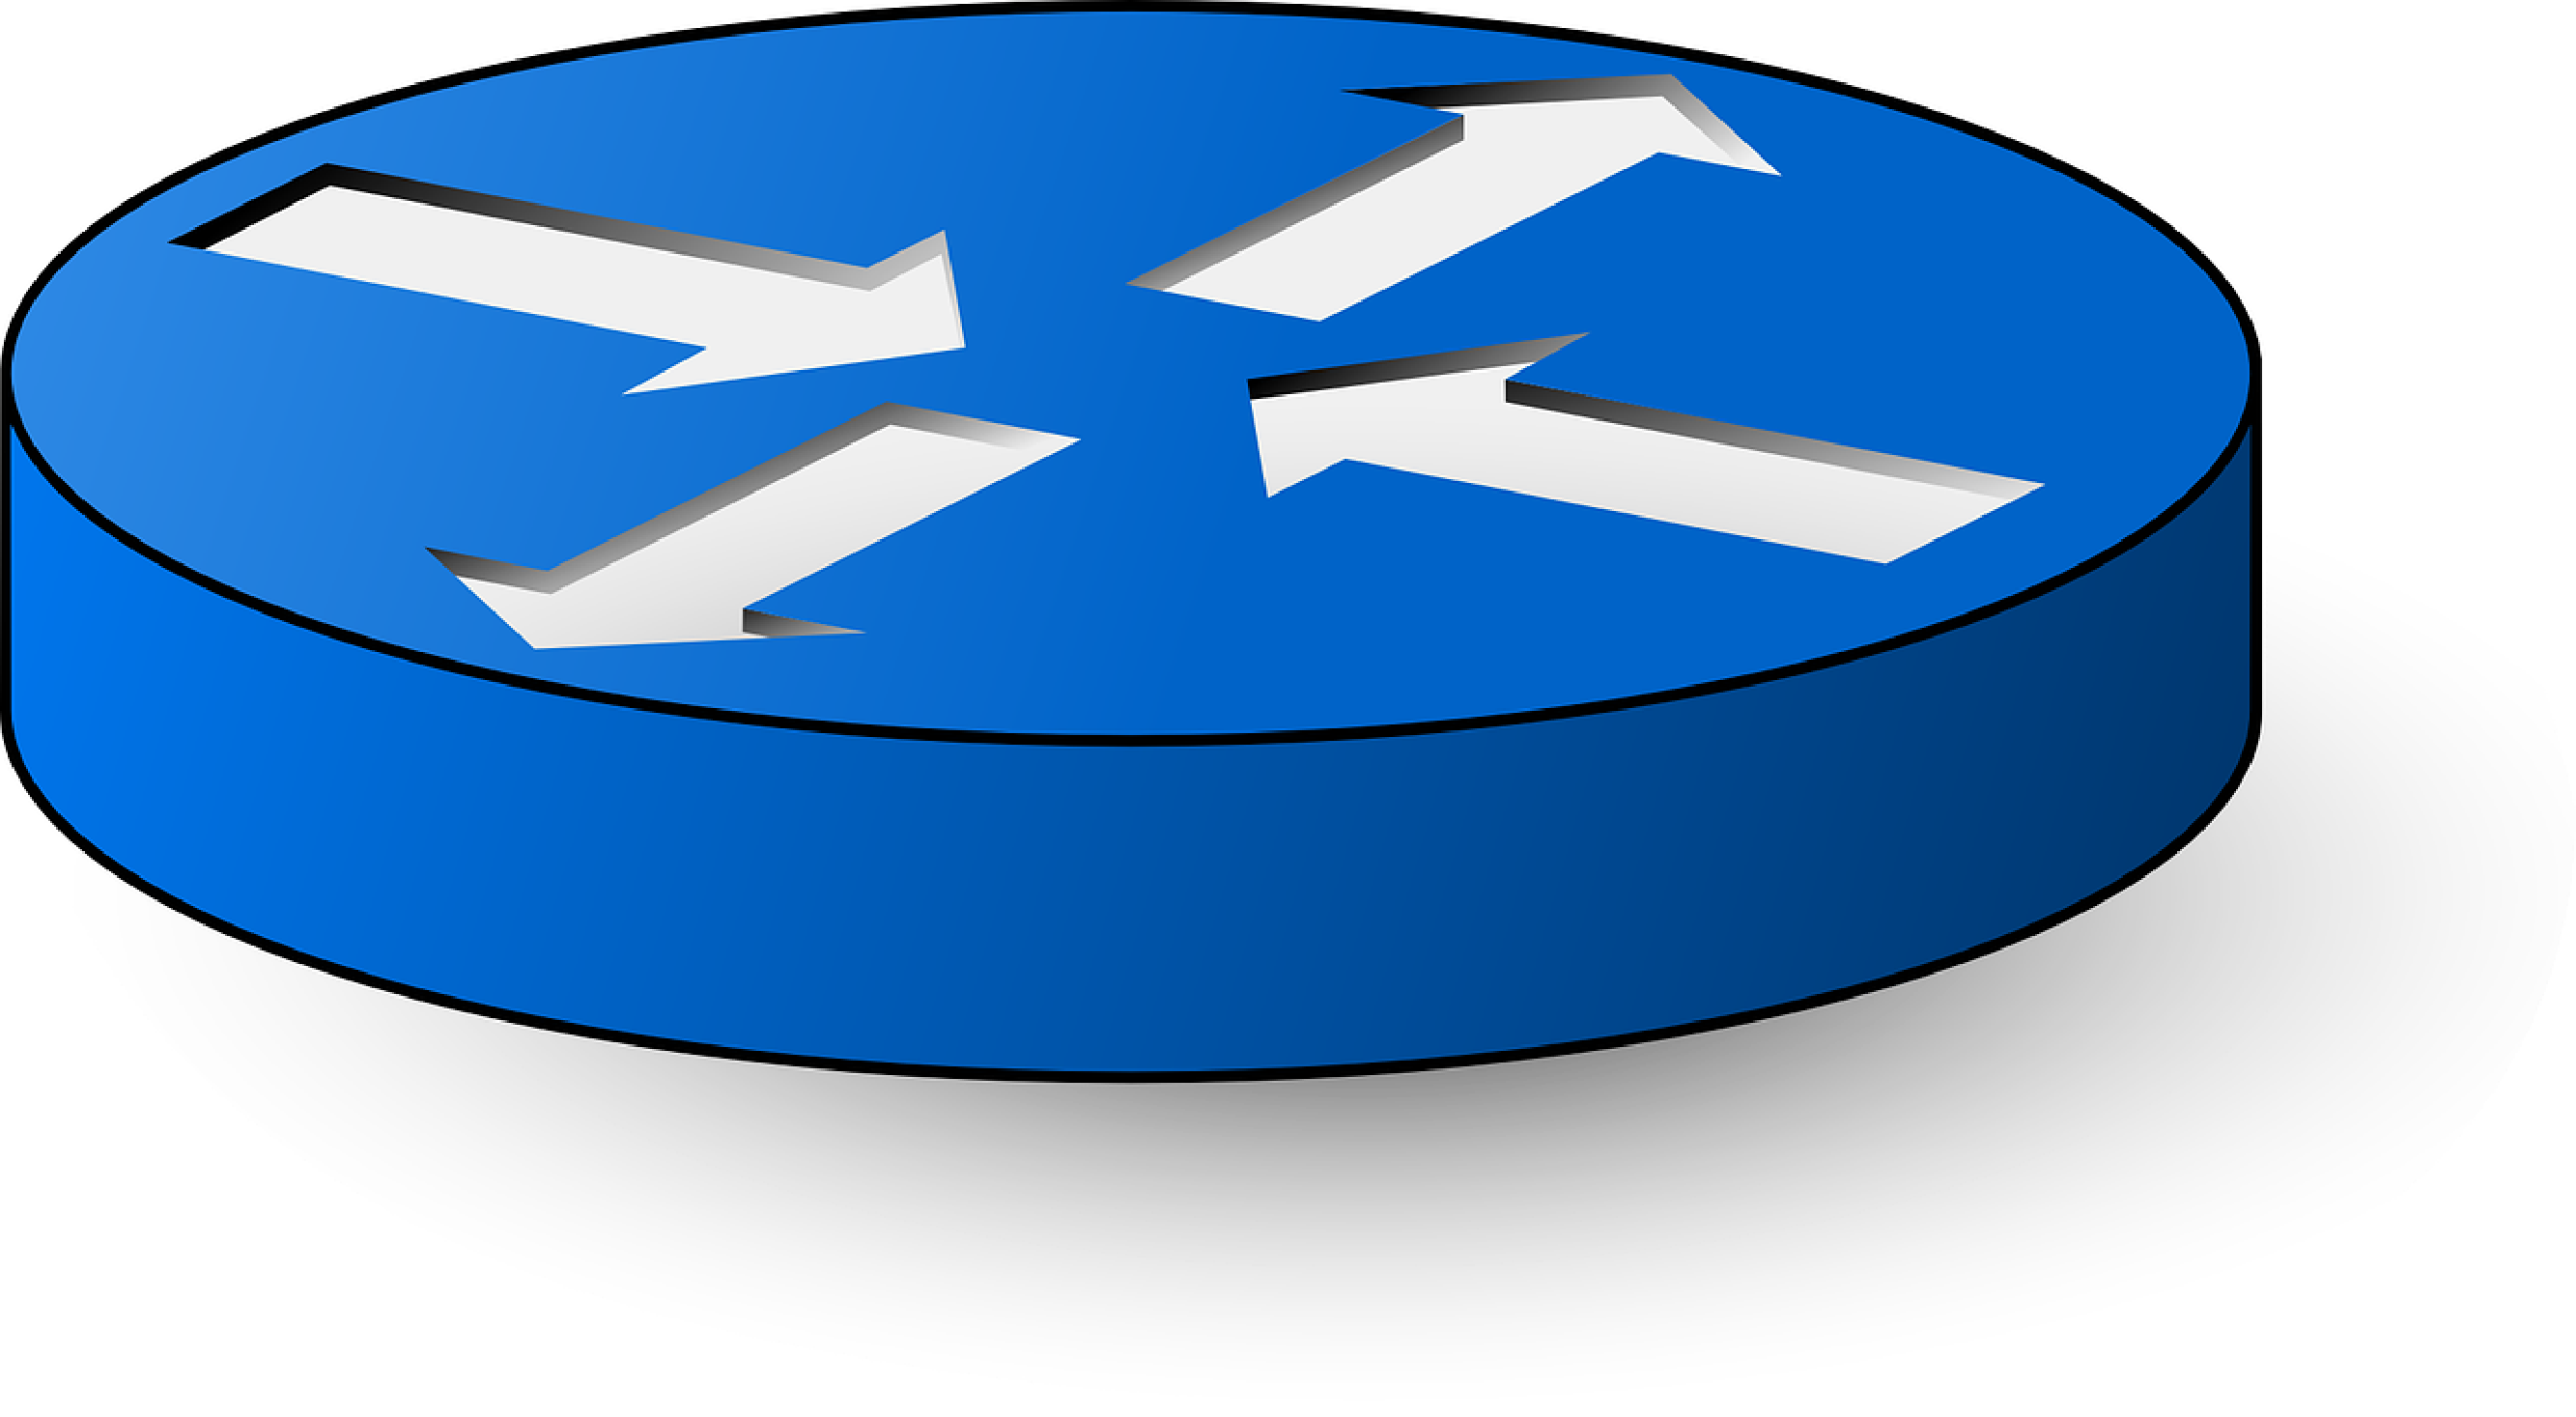
\includegraphics[width=52.5pt,height=52.5pt]{figures/router-30140_1280.pdf}};
%Image [id:dp9757131158412626] 
\draw (441.5,544.5) node  {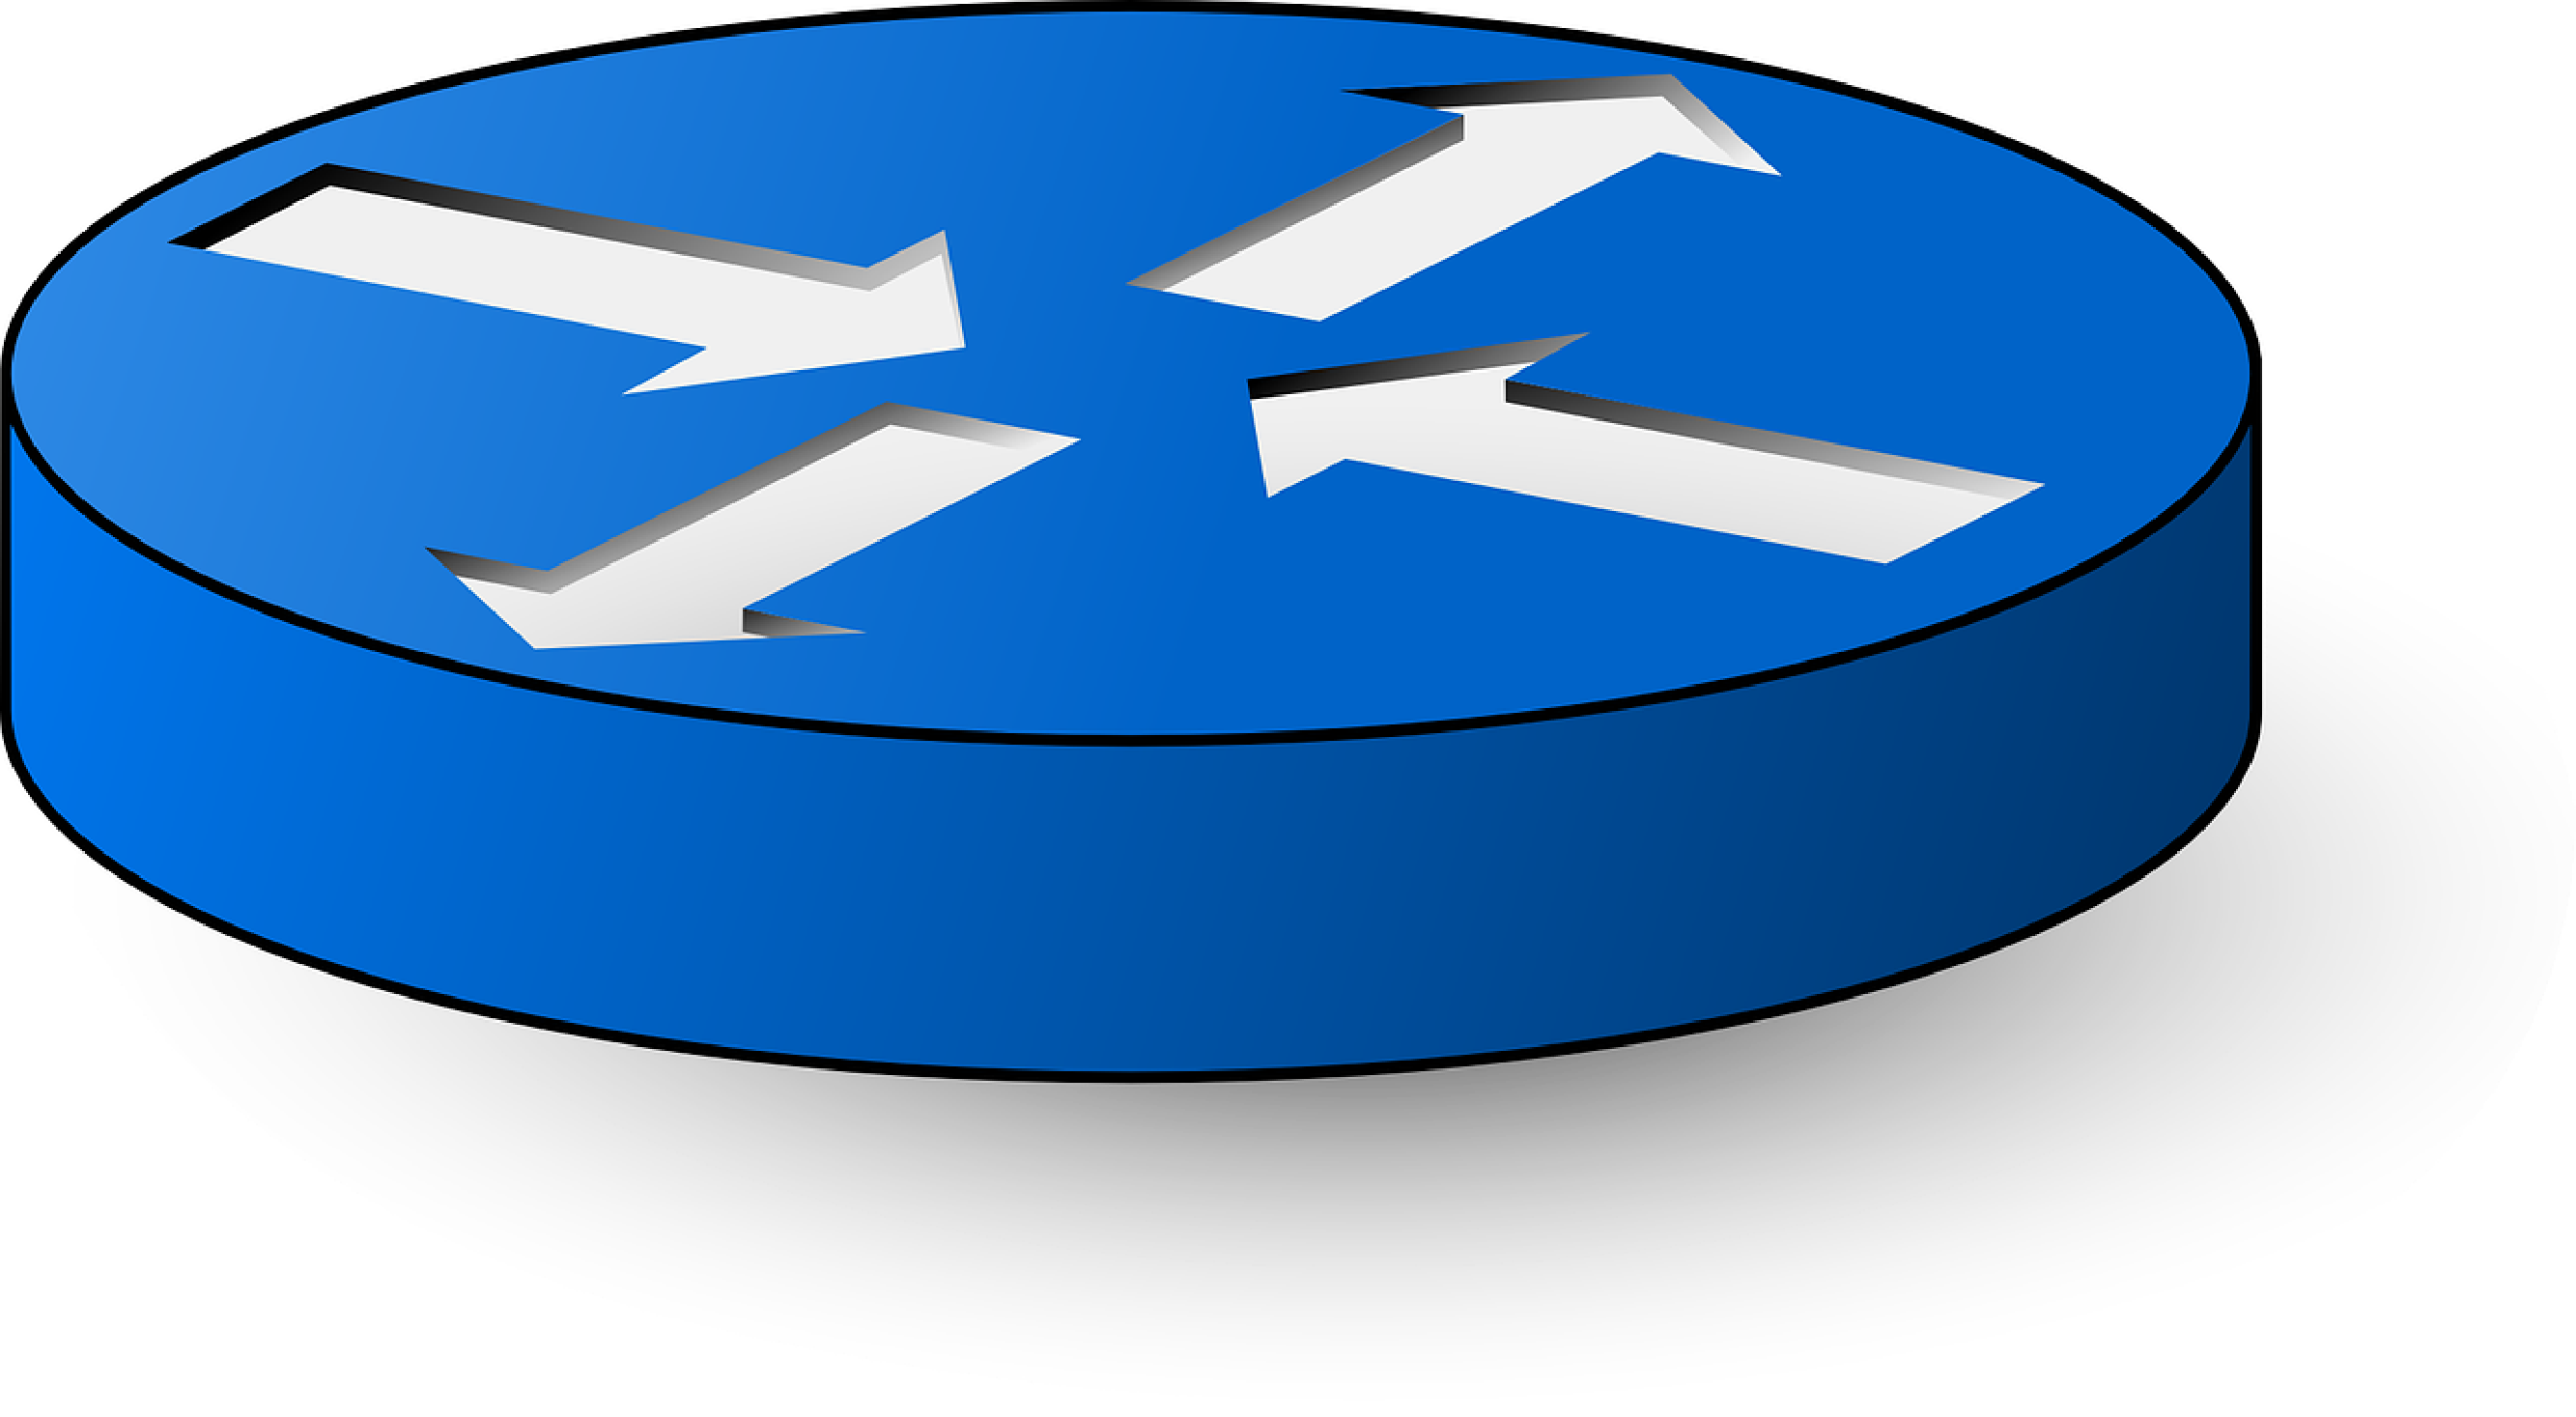
\includegraphics[width=52.5pt,height=52.5pt]{figures/router-30140_1280.pdf}};
%Image [id:dp21403253894649854] 
\draw (184,546.5) node  {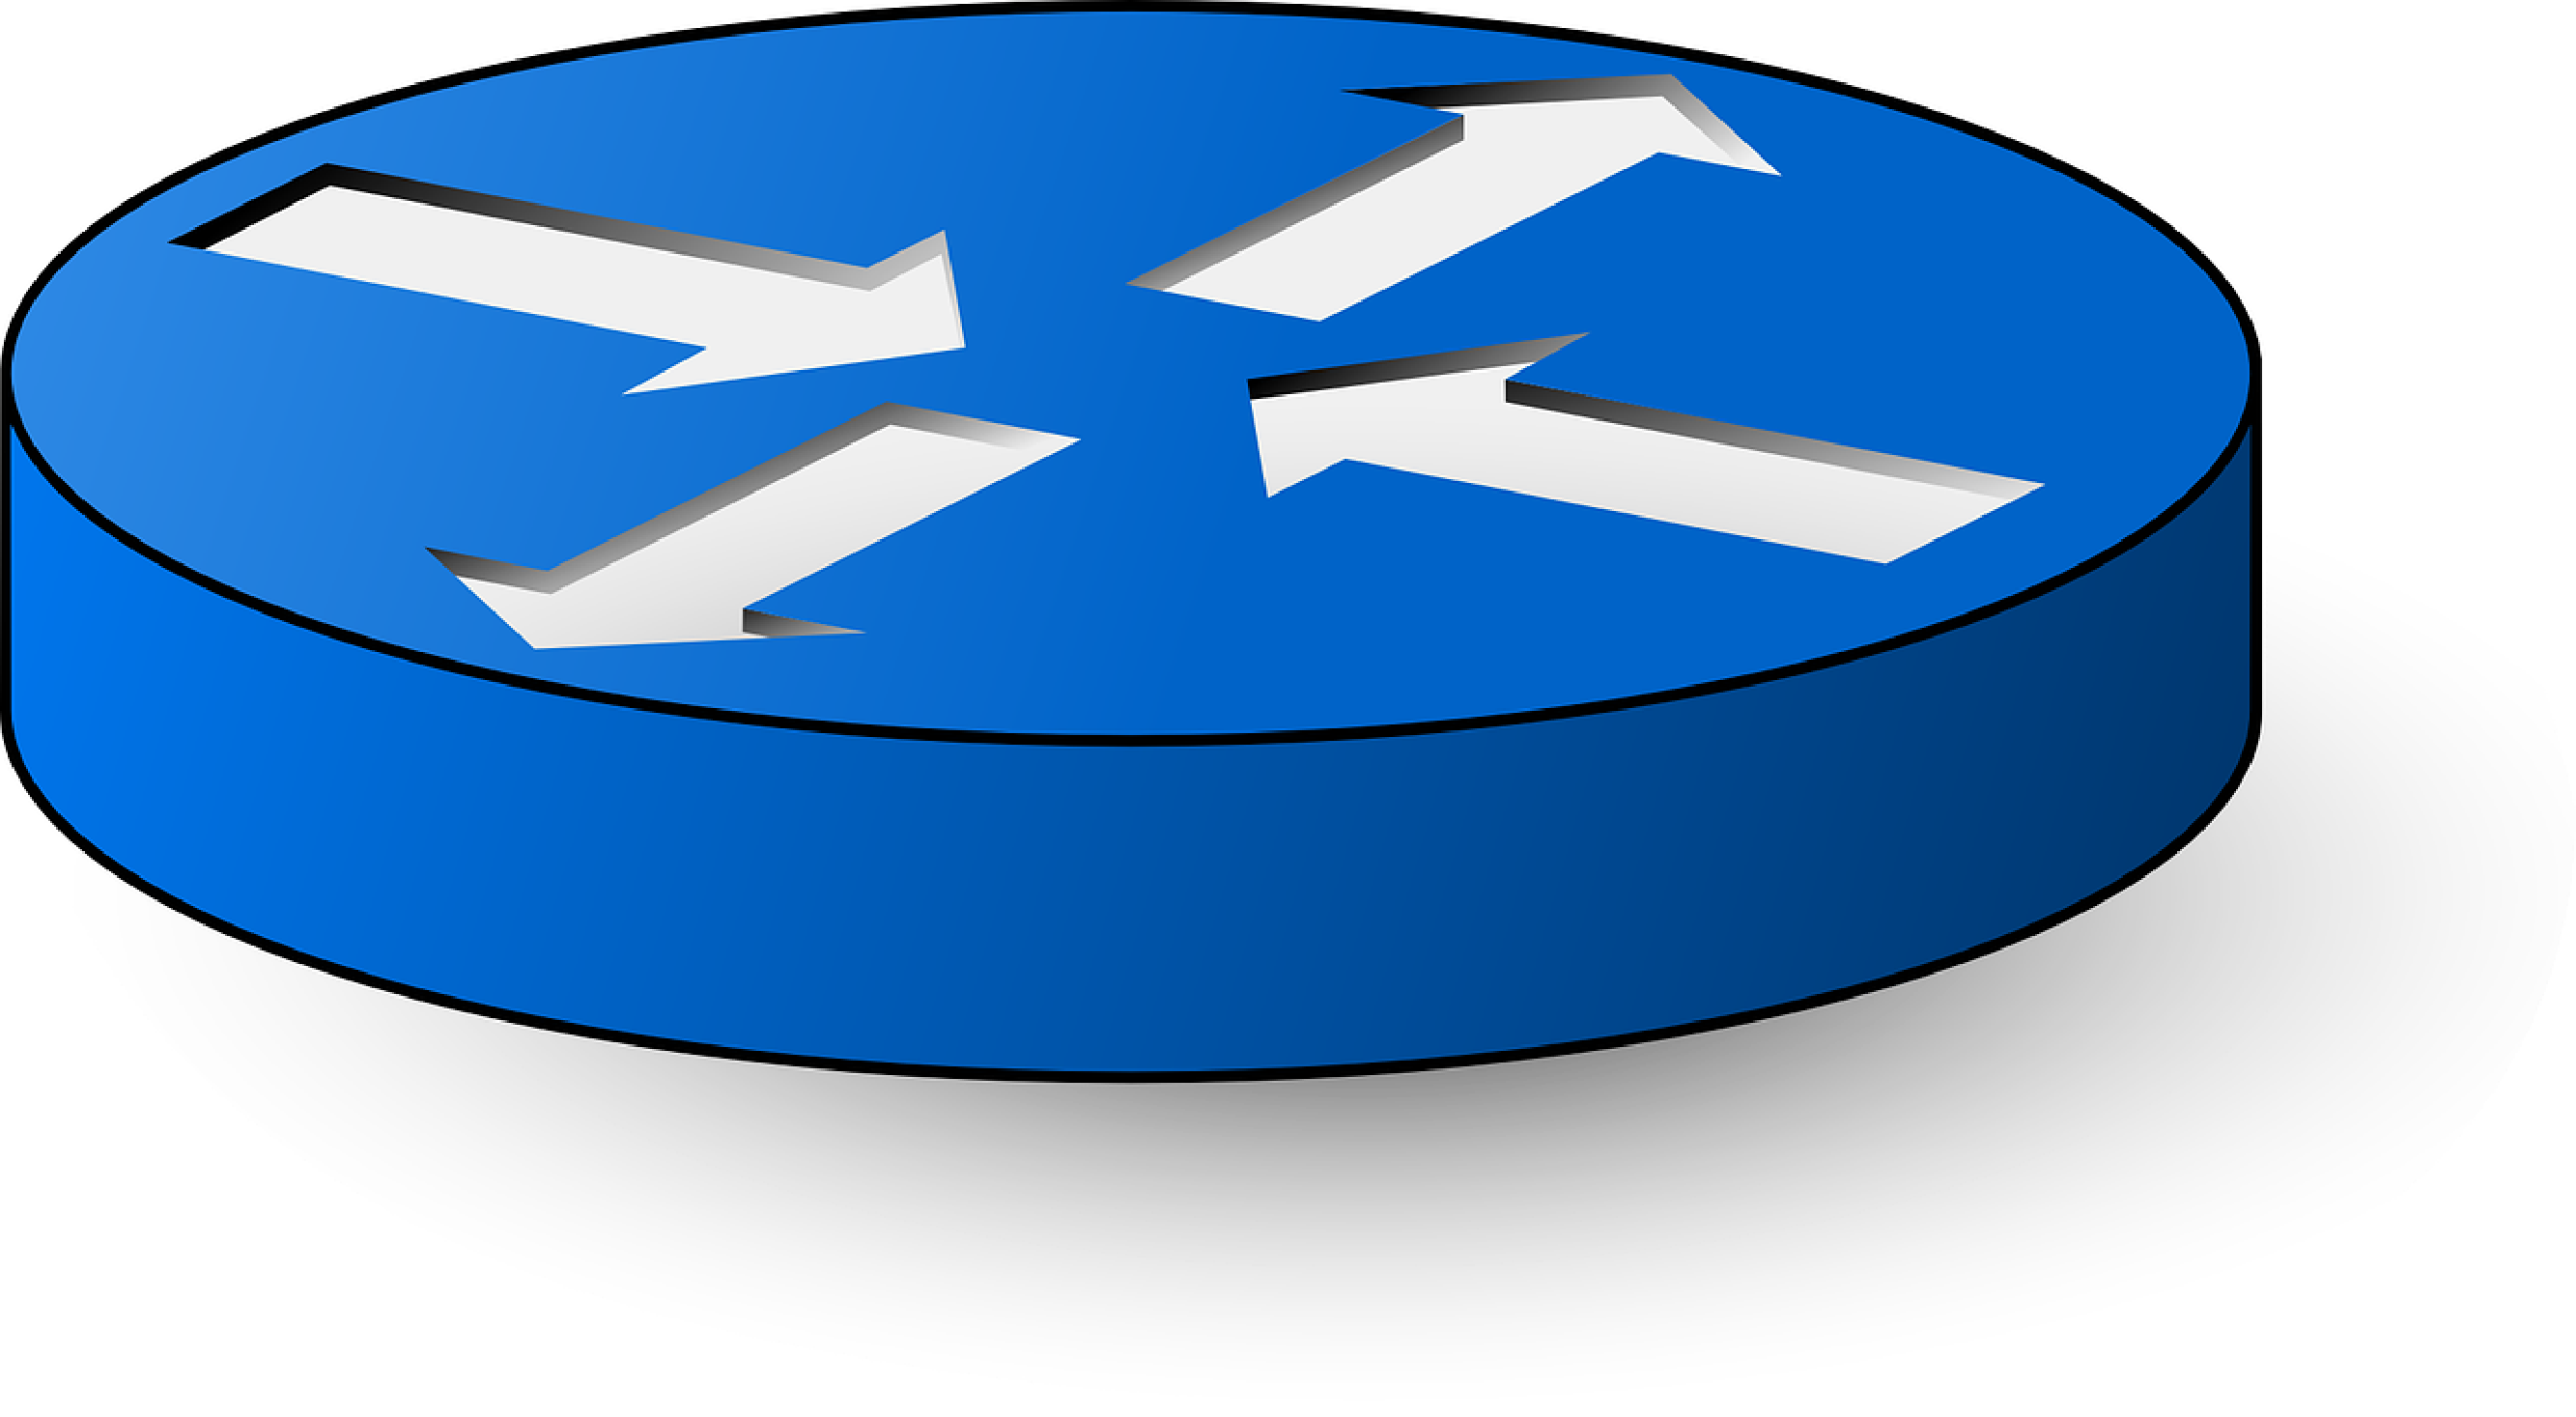
\includegraphics[width=52.5pt,height=52.5pt]{figures/router-30140_1280.pdf}};
%Image [id:dp9442712298825287] 
\draw (440.5,444.5) node  {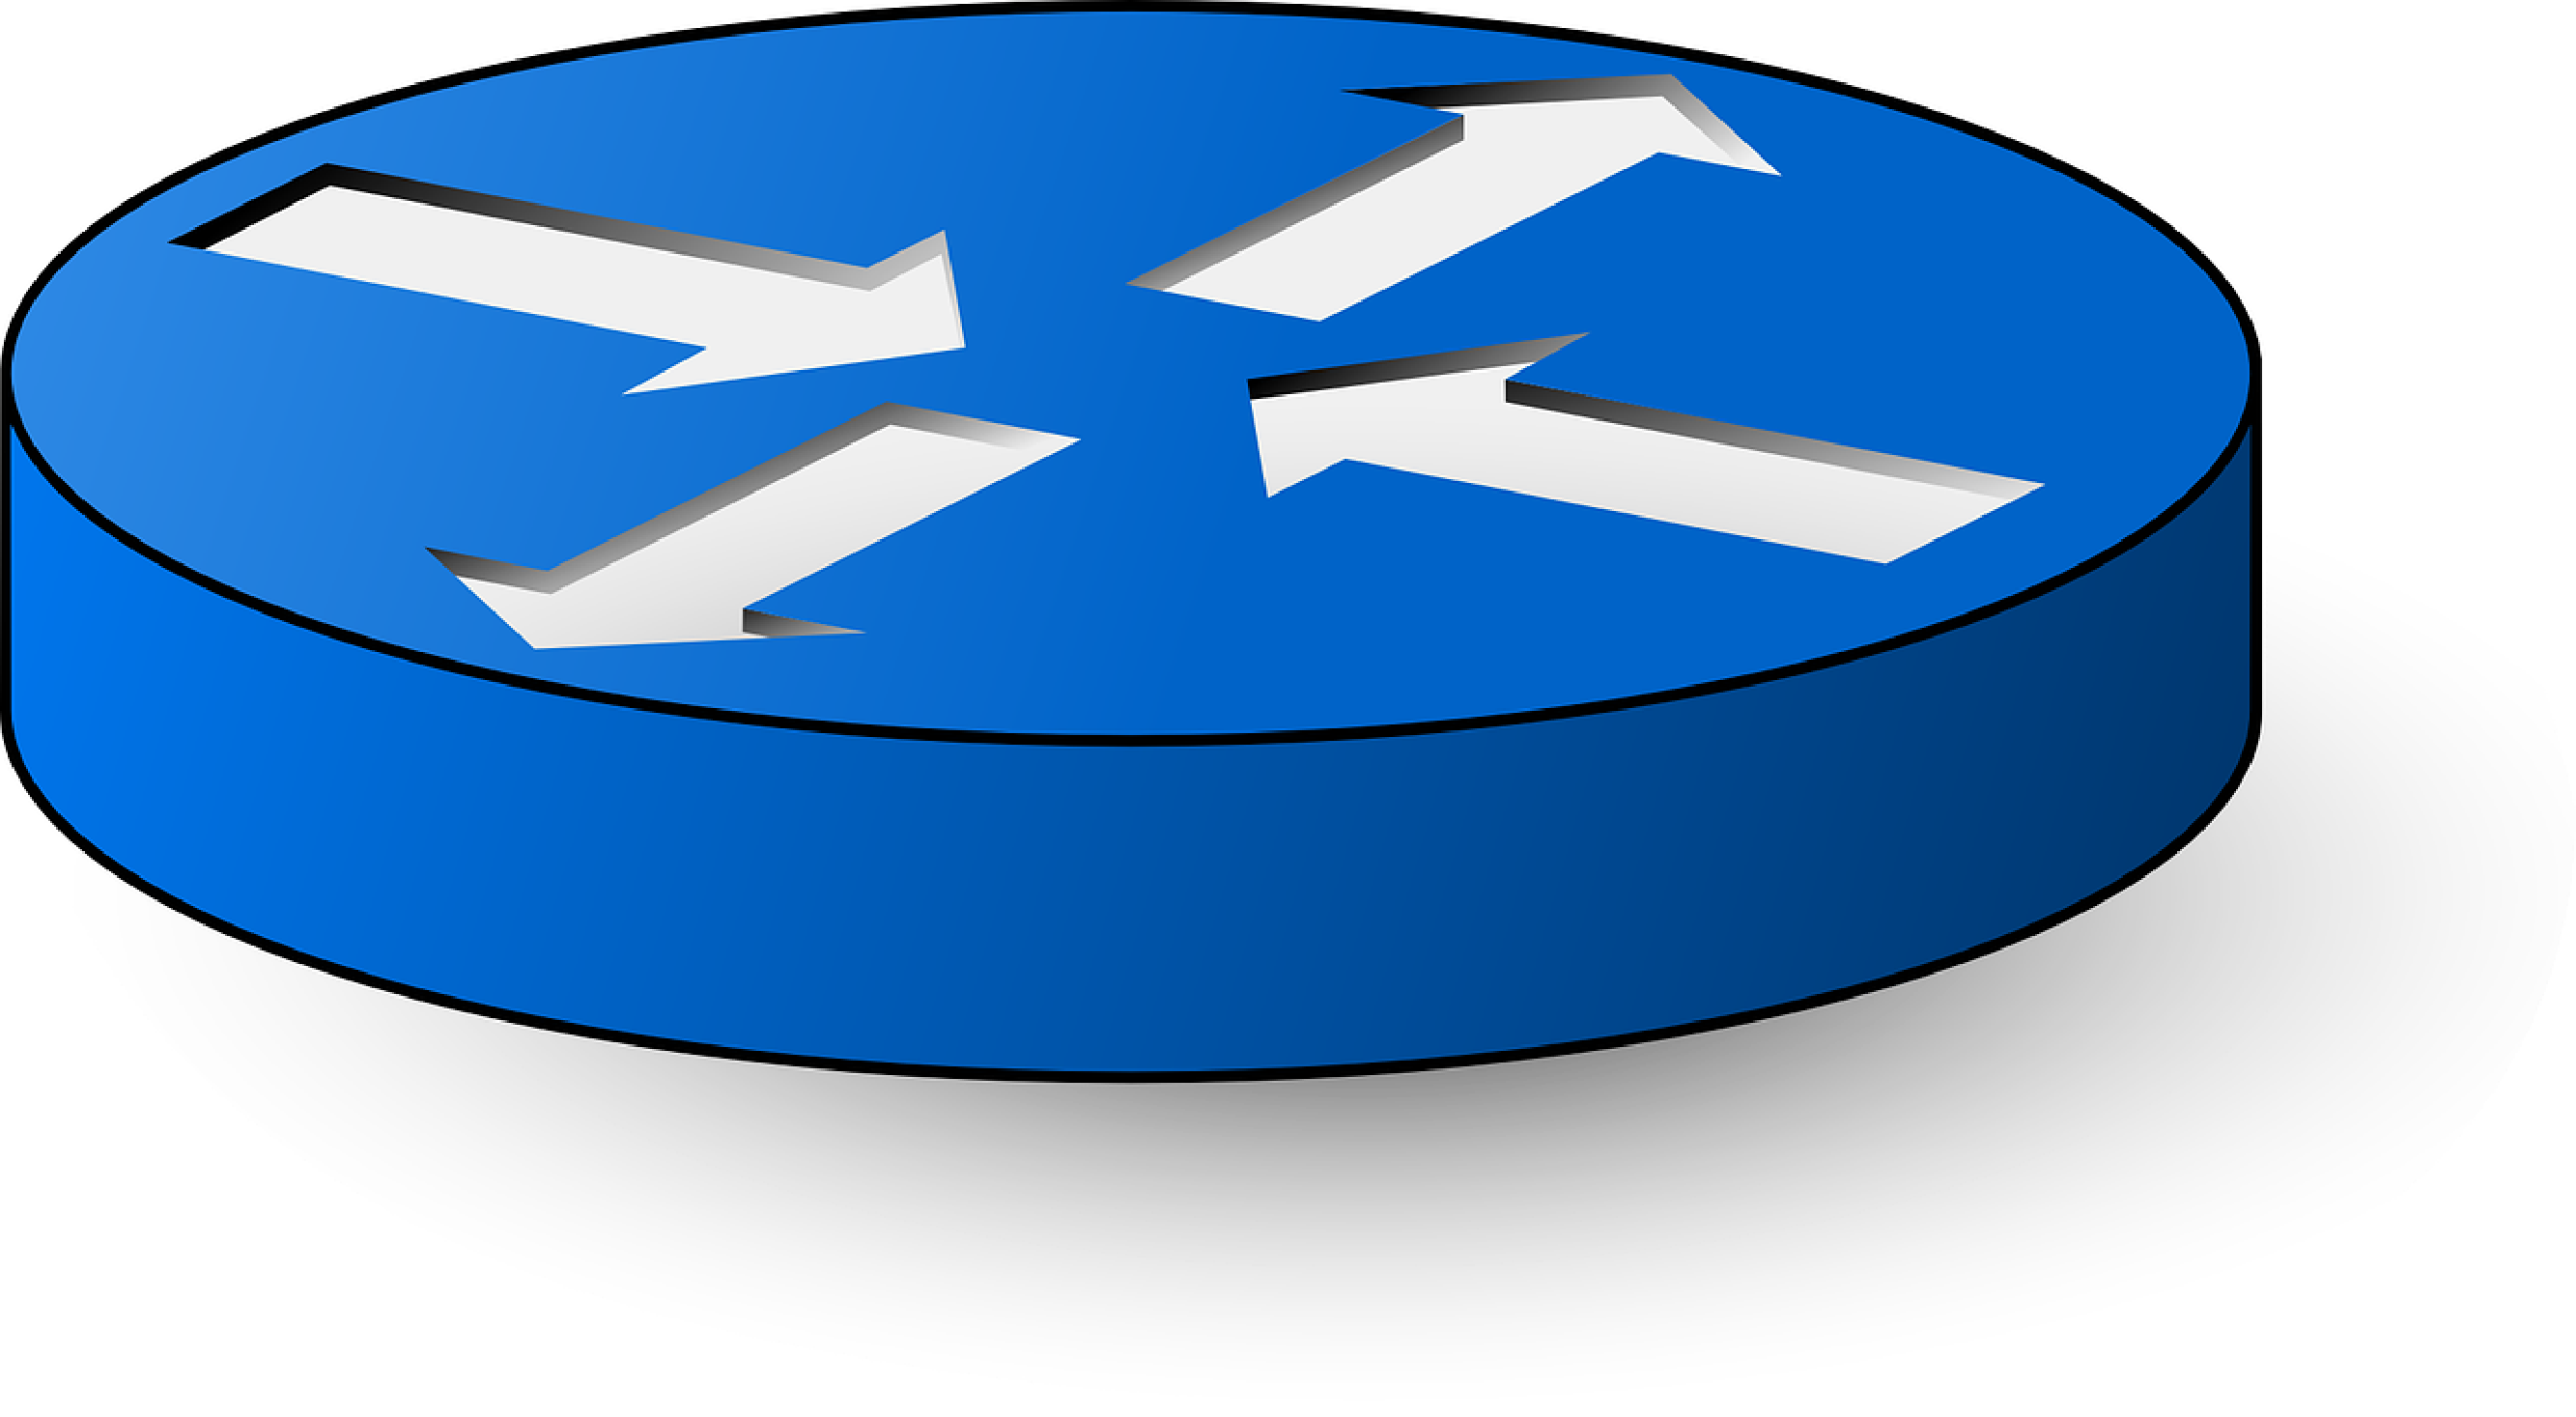
\includegraphics[width=52.5pt,height=52.5pt]{figures/router-30140_1280.pdf}};
%Straight Lines [id:da09222939335266478] 
\draw [color={rgb, 255:red, 74; green, 144; blue, 226 }  ,draw opacity=1 ][line width=1.5]    (230,333) -- (66.46,447.45) ;
\draw [shift={(64,449.17)}, rotate = 325.02] [color={rgb, 255:red, 74; green, 144; blue, 226 }  ,draw opacity=1 ][line width=1.5]    (14.21,-4.28) .. controls (9.04,-1.82) and (4.3,-0.39) .. (0,0) .. controls (4.3,0.39) and (9.04,1.82) .. (14.21,4.28)   ;

%Straight Lines [id:da6866328735169647] 
\draw [color={rgb, 255:red, 74; green, 144; blue, 226 }  ,draw opacity=1 ][line width=1.5]    (230,333) -- (432.18,405.82) ;
\draw [shift={(435,406.83)}, rotate = 199.81] [color={rgb, 255:red, 74; green, 144; blue, 226 }  ,draw opacity=1 ][line width=1.5]    (14.21,-4.28) .. controls (9.04,-1.82) and (4.3,-0.39) .. (0,0) .. controls (4.3,0.39) and (9.04,1.82) .. (14.21,4.28)   ;

%Shape: Cloud [id:dp2992812680460014] 
\draw  [fill={rgb, 255:red, 255; green, 255; blue, 255 }  ,fill opacity=1 ] (557.19,464.58) .. controls (556.29,457.33) and (559.25,450.16) .. (564.82,446.11) .. controls (570.39,442.05) and (577.58,441.82) .. (583.36,445.52) .. controls (585.4,441.31) and (589.14,438.4) .. (593.45,437.68) .. controls (597.76,436.95) and (602.13,438.5) .. (605.24,441.84) .. controls (606.98,438.02) and (610.4,435.46) .. (614.28,435.06) .. controls (618.17,434.65) and (621.97,436.47) .. (624.34,439.87) .. controls (627.48,435.82) and (632.49,434.11) .. (637.19,435.49) .. controls (641.89,436.87) and (645.44,441.08) .. (646.31,446.3) .. controls (650.16,447.45) and (653.38,450.37) .. (655.11,454.31) .. controls (656.85,458.25) and (656.94,462.82) .. (655.37,466.84) .. controls (659.17,472.24) and (660.06,479.44) .. (657.7,485.75) .. controls (655.35,492.05) and (650.11,496.52) .. (643.94,497.49) .. controls (643.9,503.41) and (640.93,508.84) .. (636.17,511.69) .. controls (631.42,514.54) and (625.63,514.36) .. (621.03,511.23) .. controls (619.07,518.32) and (613.56,523.53) .. (606.87,524.62) .. controls (600.18,525.71) and (593.52,522.48) .. (589.76,516.32) .. controls (585.16,519.36) and (579.63,520.23) .. (574.43,518.75) .. controls (569.23,517.27) and (564.8,513.55) .. (562.12,508.44) .. controls (557.42,509.04) and (552.87,506.37) .. (550.73,501.76) .. controls (548.6,497.16) and (549.33,491.58) .. (552.57,487.81) .. controls (548.37,485.11) and (546.23,479.75) .. (547.26,474.53) .. controls (548.29,469.31) and (552.26,465.41) .. (557.1,464.86) ; \draw   (552.57,487.81) .. controls (554.55,489.09) and (556.84,489.67) .. (559.13,489.47)(562.12,508.44) .. controls (563.11,508.31) and (564.07,508.04) .. (564.99,507.64)(589.76,516.32) .. controls (589.07,515.19) and (588.49,513.97) .. (588.04,512.7)(621.03,511.23) .. controls (621.39,509.94) and (621.62,508.6) .. (621.72,507.26)(643.94,497.49) .. controls (643.99,491.19) and (640.71,485.42) .. (635.52,482.66)(655.37,466.84) .. controls (654.53,468.99) and (653.24,470.89) .. (651.62,472.4)(646.31,446.3) .. controls (646.45,447.16) and (646.52,448.04) .. (646.5,448.93)(624.34,439.87) .. controls (623.55,440.87) and (622.91,442) .. (622.42,443.21)(605.24,441.84) .. controls (604.82,442.76) and (604.51,443.73) .. (604.31,444.73)(583.36,445.52) .. controls (584.58,446.3) and (585.71,447.24) .. (586.72,448.32)(557.19,464.58) .. controls (557.32,465.58) and (557.51,466.56) .. (557.78,467.53) ;
%Straight Lines [id:da885478252254038] 
\draw [line width=1.5]  [dash pattern={on 1.69pt off 2.76pt}]  (450.5,82.33) -- (489.5,82.83) ;


%Straight Lines [id:da6105591508346683] 
\draw    (450,98.71) -- (490,99.21) ;


%Straight Lines [id:da021279170004724568] 
\draw [color={rgb, 255:red, 74; green, 144; blue, 226 }  ,draw opacity=1 ][line width=1.5]    (453.5,131.13) -- (483.5,130.97) ;
\draw [shift={(486.5,130.96)}, rotate = 539.71] [color={rgb, 255:red, 74; green, 144; blue, 226 }  ,draw opacity=1 ][line width=1.5]    (14.21,-4.28) .. controls (9.04,-1.82) and (4.3,-0.39) .. (0,0) .. controls (4.3,0.39) and (9.04,1.82) .. (14.21,4.28)   ;

%Rounded Rect [id:dp201331626843132] 
\draw  [fill={rgb, 255:red, 217; green, 154; blue, 232 }  ,fill opacity=1 ] (6,294.78) .. controls (6,289.88) and (9.98,285.9) .. (14.89,285.9) -- (500.11,285.9) .. controls (505.02,285.9) and (509,289.88) .. (509,294.78) -- (509,321.45) .. controls (509,326.35) and (505.02,330.33) .. (500.11,330.33) -- (14.89,330.33) .. controls (9.98,330.33) and (6,326.35) .. (6,321.45) -- cycle ;

%Shape: Polygon Curved [id:ds08242749430225138] 
\draw  [color={rgb, 255:red, 255; green, 248; blue, 177 }  ,draw opacity=1 ][line width=2.25]  (41,423.33) .. controls (61,413.33) and (210,392.33) .. (232,407.33) .. controls (254,422.33) and (264,544.33) .. (248,574.33) .. controls (232,604.33) and (53.5,538.83) .. (33.5,508.83) .. controls (13.5,478.83) and (21,433.33) .. (41,423.33) -- cycle ;
%Straight Lines [id:da08659205633415445] 
\draw [color={rgb, 255:red, 255; green, 255; blue, 139 }  ,draw opacity=1 ][line width=2.25]    (450,147.71) -- (490,148.21) ;


%Straight Lines [id:da012161855616681594] 
\draw [color={rgb, 255:red, 242; green, 175; blue, 175 }  ,draw opacity=1 ][line width=2.25]    (450,167.71) -- (490,168.21) ;



% Text Node
\draw (55,240) node  [align=left] {(A1)};
% Text Node
\draw (211,471) node  [align=left] {(A3)};
% Text Node
\draw (113,594) node  [align=left] {Physical Infrastructure};
% Text Node
\draw (599,474) node  [align=left] {Internet};
% Text Node
\draw (417,198) node  [align=left] {(A2)};
% Text Node
\draw (587,501) node  [align=left] {(A4)};
% Text Node
\draw (536,82) node  [align=left] {Virtual Link};
% Text Node
\draw (543,103) node  [align=left] {Physical Link};
% Text Node
\draw (577,125) node  [align=left] {Hypervisor - Switch link};
% Text Node
\draw (563,148) node  [align=left] {vSDN1 Embedding};
% Text Node
\draw (564,169) node  [align=left] {vSDN2 Embedding};
% Text Node
\draw (257.5,308.11) node  [align=left] {Network Hypervisor};
% Text Node
\draw (55.76,94.79) node  [align=left] {{\small vSDN1}};
% Text Node
\draw (282.98,198.5) node [scale=0.9] [align=left] {{\small vSDN2}};


\end{tikzpicture}

\caption{Attack surface of the SDN environment}
\label{fig:attack-surface}
\end{figure}